% Copyright (c) 2014,2016,2018 Casper Ti. Vector
% Public domain.

\chapter{exFAT文件系统的设计与实现}
%\pkuthssffaq % 中文测试文字。
本研究实现的 exFAT 文件系统可以划分成以下几个相对独立模块:文件系统的中枢部分、FAT表及文件的分配与访问、目录的解析、
大写转换表、Bitmap、索引节点实现,各个模块之间存在交互。
其中文件系统的中枢部分是文件系统的核心,里面包括了exFAT的所有组件的实例,
并对外提供和整个文件系统相关的接口。
索引节点(Index node,本文中简称为 Inode)实现了和单个文件或文件夹相关的功能,对外提供和单个文件或文件夹操作相关的接口。
其他部分不对外提供接口,仅在文件系统内部使用。
图\ref{fig:exfat_arch}是我们实现的exFTA的总架构图。

\begin{figure}[h]
    \centering
    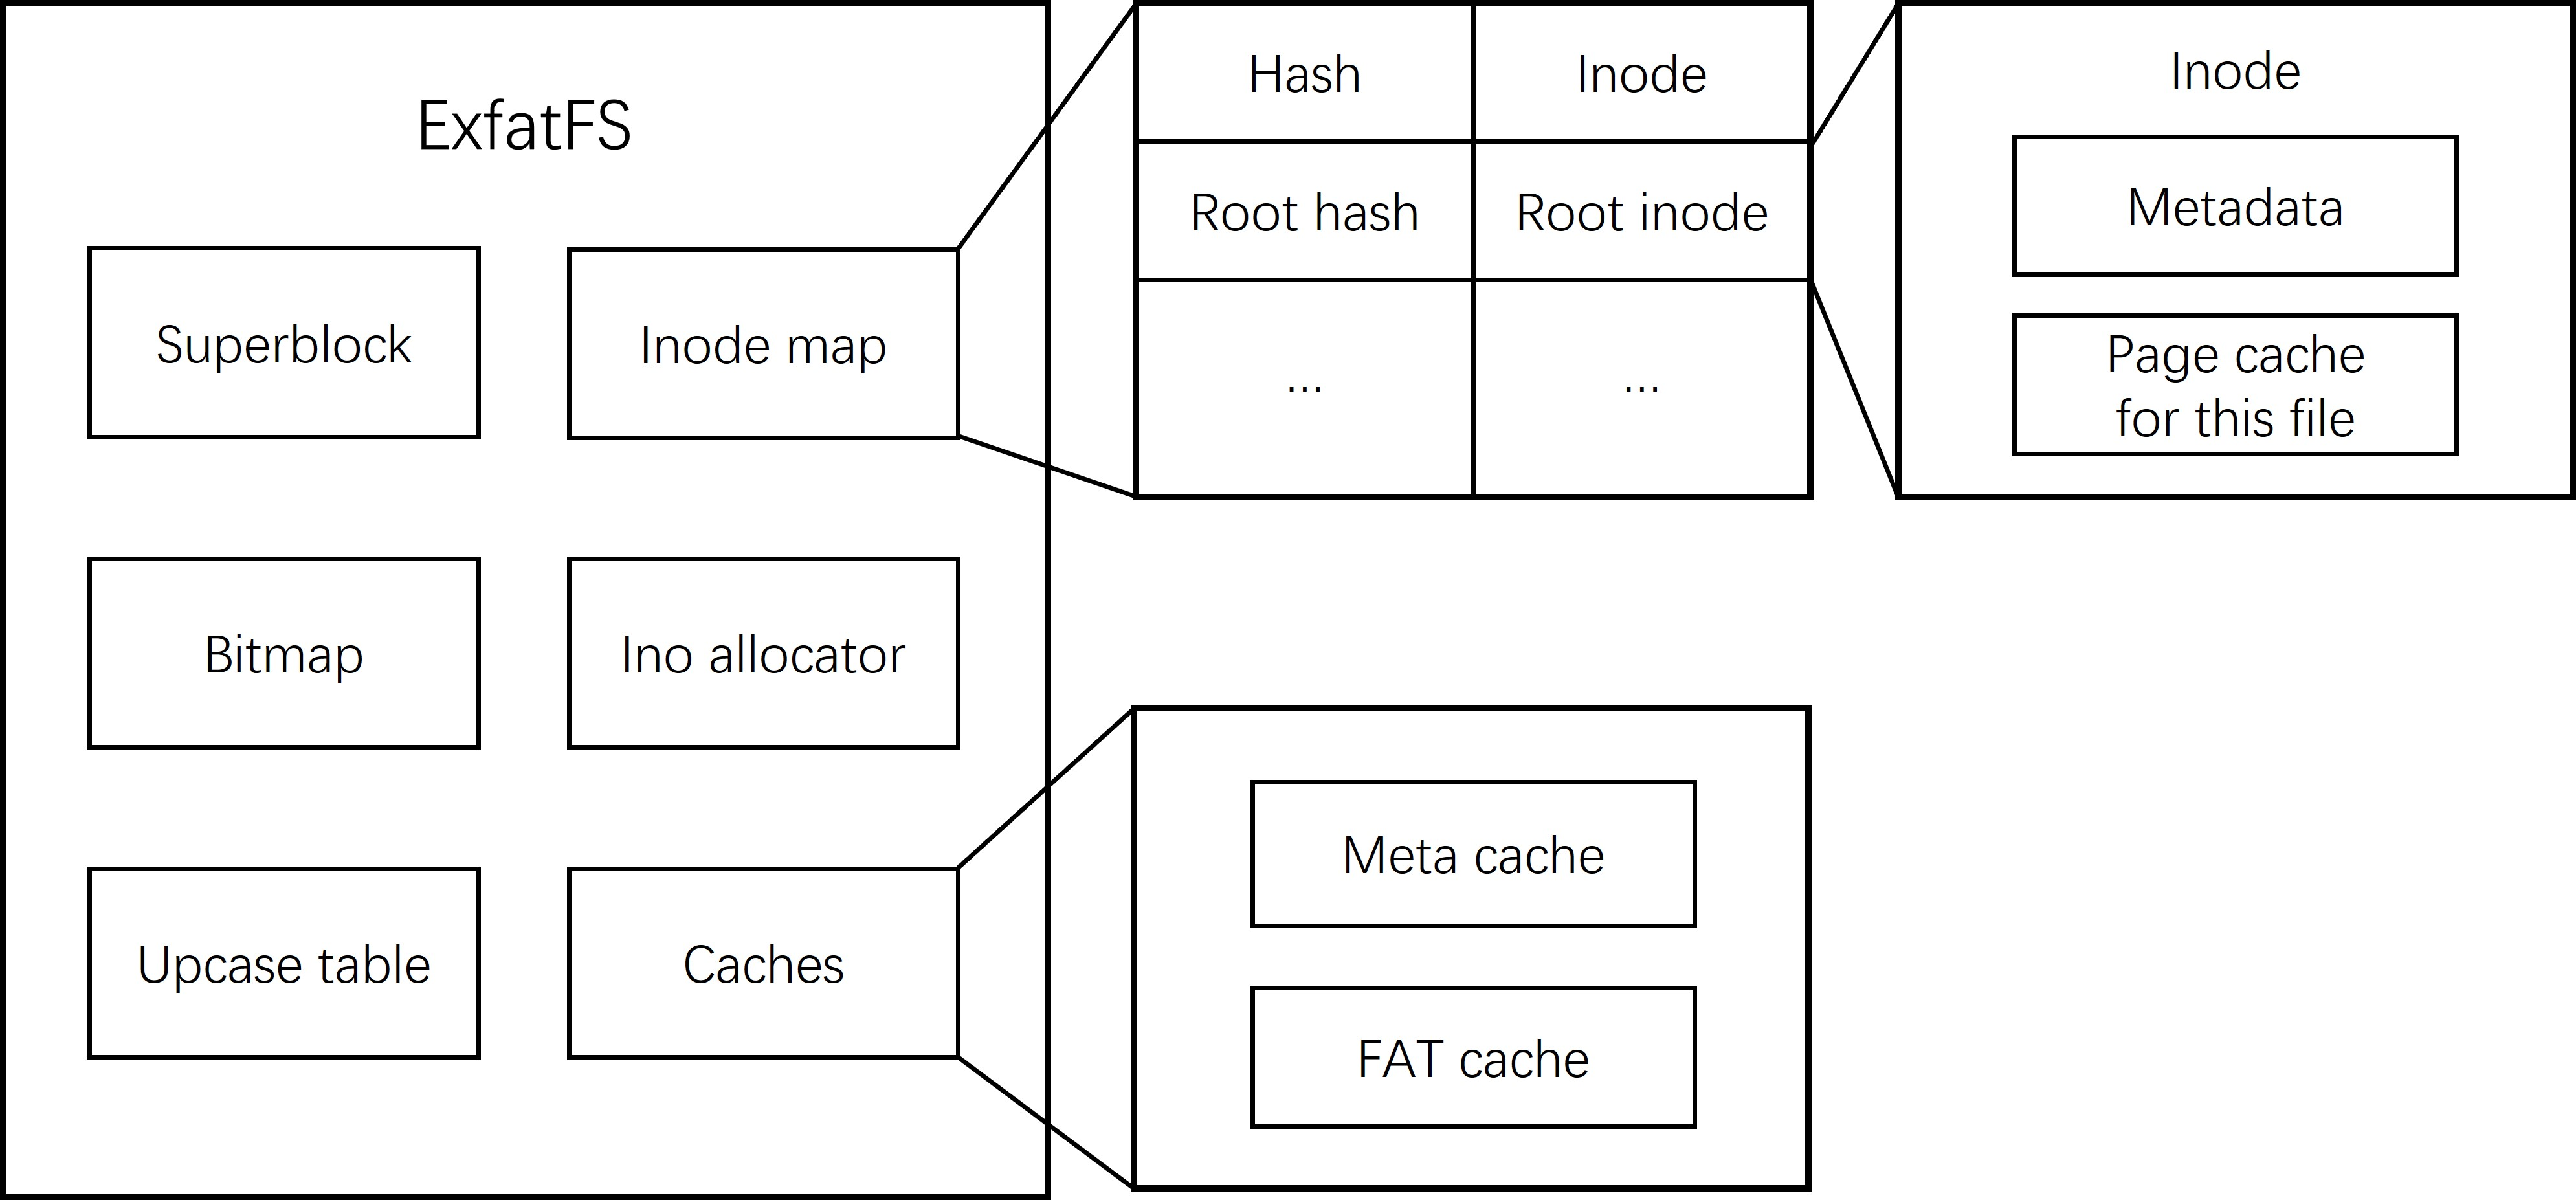
\includegraphics[width=1.0\textwidth]{chap3_exfat_arch.jpg}
    \caption{exFAT总架构}
    \label{fig:exfat_arch}
\end{figure}
\section{文件系统的中枢部分}
文件系统的中枢部分被实现为图\ref{fig:exfat_arch}中的结构体 ExfatFS,这个结构体会在 exFTA 被挂载时创建,伴随 exFAT 直至其被取消挂载。
ExfatFS 中的首要功能就是挂载 exFAT 文件系统。
exFAT 被挂载时会首先从块设备上读取超级块,若发现位于起始位置的超级块受损,
系统会尝试读取后备超级块。当系统读取到正确的超级块后,可以从其中获取文件系统的基本信息,
包括扇区和簇的大小和数量、根目录所在簇、FAT区的起始扇区和数据区的起始扇区。
随后,系统会根据根目录所在簇打开根目录,建立根目录的索引节点(Root inode)。
根目录的 Inode 被分配到 Inode 编号是 1,这也是最小的 Inode 编号。
接着,系统会在根目录中寻找 Bitmap 目录项和 Upcase Table 目录项,分别初始化 Bitmap 和大写转换表。
至此,exFAT 文件系统挂载完成。

ExfatFS 作为文件系统的中枢部分,负责管理所有打开的Inode和分配Inode编号(Inode number,本文中简称Ino)。
每打开一个新的Inode,ExfatFS 的Ino分配器(Ino allocator)会为其分配一个新的编号。
Ino分配器被实现为一个支持原子操作的64位无符号数,维护下一个要分配的 Ino。
当需要分配新的Ino时,Ino分配器会进行自增,并返回自增前的值作为分配结果。
ExfatFS 使用一个 HashMap 管理打开的Inode,如图\ref{fig:exfat_arch}中的Inode map所示。
使用 HashMap 的目的是能通过文件相关信息计算出哈希值,从而直接找到对应的Inode。
哈希值的选择应该满足在整个 exFAT 文件系统中唯一,故不能使用文件名的字符串哈希做哈希值。
完整路径名的字符串哈希是一个可行的选择,但可能存在潜在的哈希值碰撞的情况。
我们的设计中采用了另一种计算哈希值的方式,如式\ref{eq:hash}所示,使用某文件对应的目录项集的主目录项的位置来计算哈希值
(唯一的特例是根目录,根目录不存在关联的目录项),这种计算方式显然可确保唯一性,而且也不存在碰撞的可能。
\begin{equation}\label{eq:hash}
    hash(inode) = 
    \begin{cases}
        root\_hash & \text{root inode} \\
        (pos.cluster\_id \ll 32) \text{ }|\text{ } pos.offset & \text{other inode}
    \end{cases}
\end{equation}
在元数据管理方面,ExfatFS 使用了两个 Cache 来缓存与管理 exFAT 中涉及的元数据。
第一个 Cache (Meta cache)是一个普通的页缓存,按页粒度缓存 exFAT 中元数据相关的页面,
这可能包括FAT区的页面、系统文件 Bitmap 和大写转换表中的页面等。
为了方便访问FAT表,我们还使用了另一个 Cache,第二个 Cache (FAT cache)是一个基于LRU的 Cache,
缓存粒度是具体的FAT表项,Cache 中的每个条目都代表单个FAT映射。

\section{FAT表及文件的分配与访问}\label{sec:FAT}
exFTA文件系统的所有文件和目录数据都存储在位于数据区的簇堆中,簇堆是一系列的簇的集合。
数据的位置可以通过一个二元组(簇的编号 Cluster id,簇内偏置 offset)唯一确定。

exFAT允许的文件分配方式有两种:连续分配和使用FAT表分配。
连续分配不使用FAT表,使用这种分配方式的文件会在目录项中给出文件起始簇的编号和文件的大小,
访问文件内容的过程无需查找FAT表。
使用FAT表分配的方式将文件内容组织成一系列的簇链,通过FAT表可以获取当前簇的下一个簇编号,
访问文件内容的过程需要从文件起始簇不断通过查询FAT表到达访问的位置。
exFAT引入连续分配模式的目的主要是为了加速文件内寻址的过程。
很显然,只要存储空间足够,我们总可以使用FAT表进行文件的分配和组织,
而连续分配需要保证存在足够大的连续空闲空间,这一点可以通过查找 Bitmap 获得。
我们实现的exFAT文件系统的分配逻辑可以总结为:优先连续分配模式,优先不改变分配模式。
对于一个从零分配的文件,我们会首先尝试连续分配,若此时的空闲簇不满足连续分配的条件,则转向使用FAT表的分配模式。
至于扩展一个已分配文件的大小,若该文件的分配方式是使用FAT表分配,则保持分配方式不变即可;
若该文件的分配方式是连续分配,则会首先尝试继续使用连续分配,从文件末尾处扩展文件,如果无法延续,
则转向使用FAT表的分配模式并为已分配的部分补充填写FAT表。

\begin{figure}[h]
    \centering
    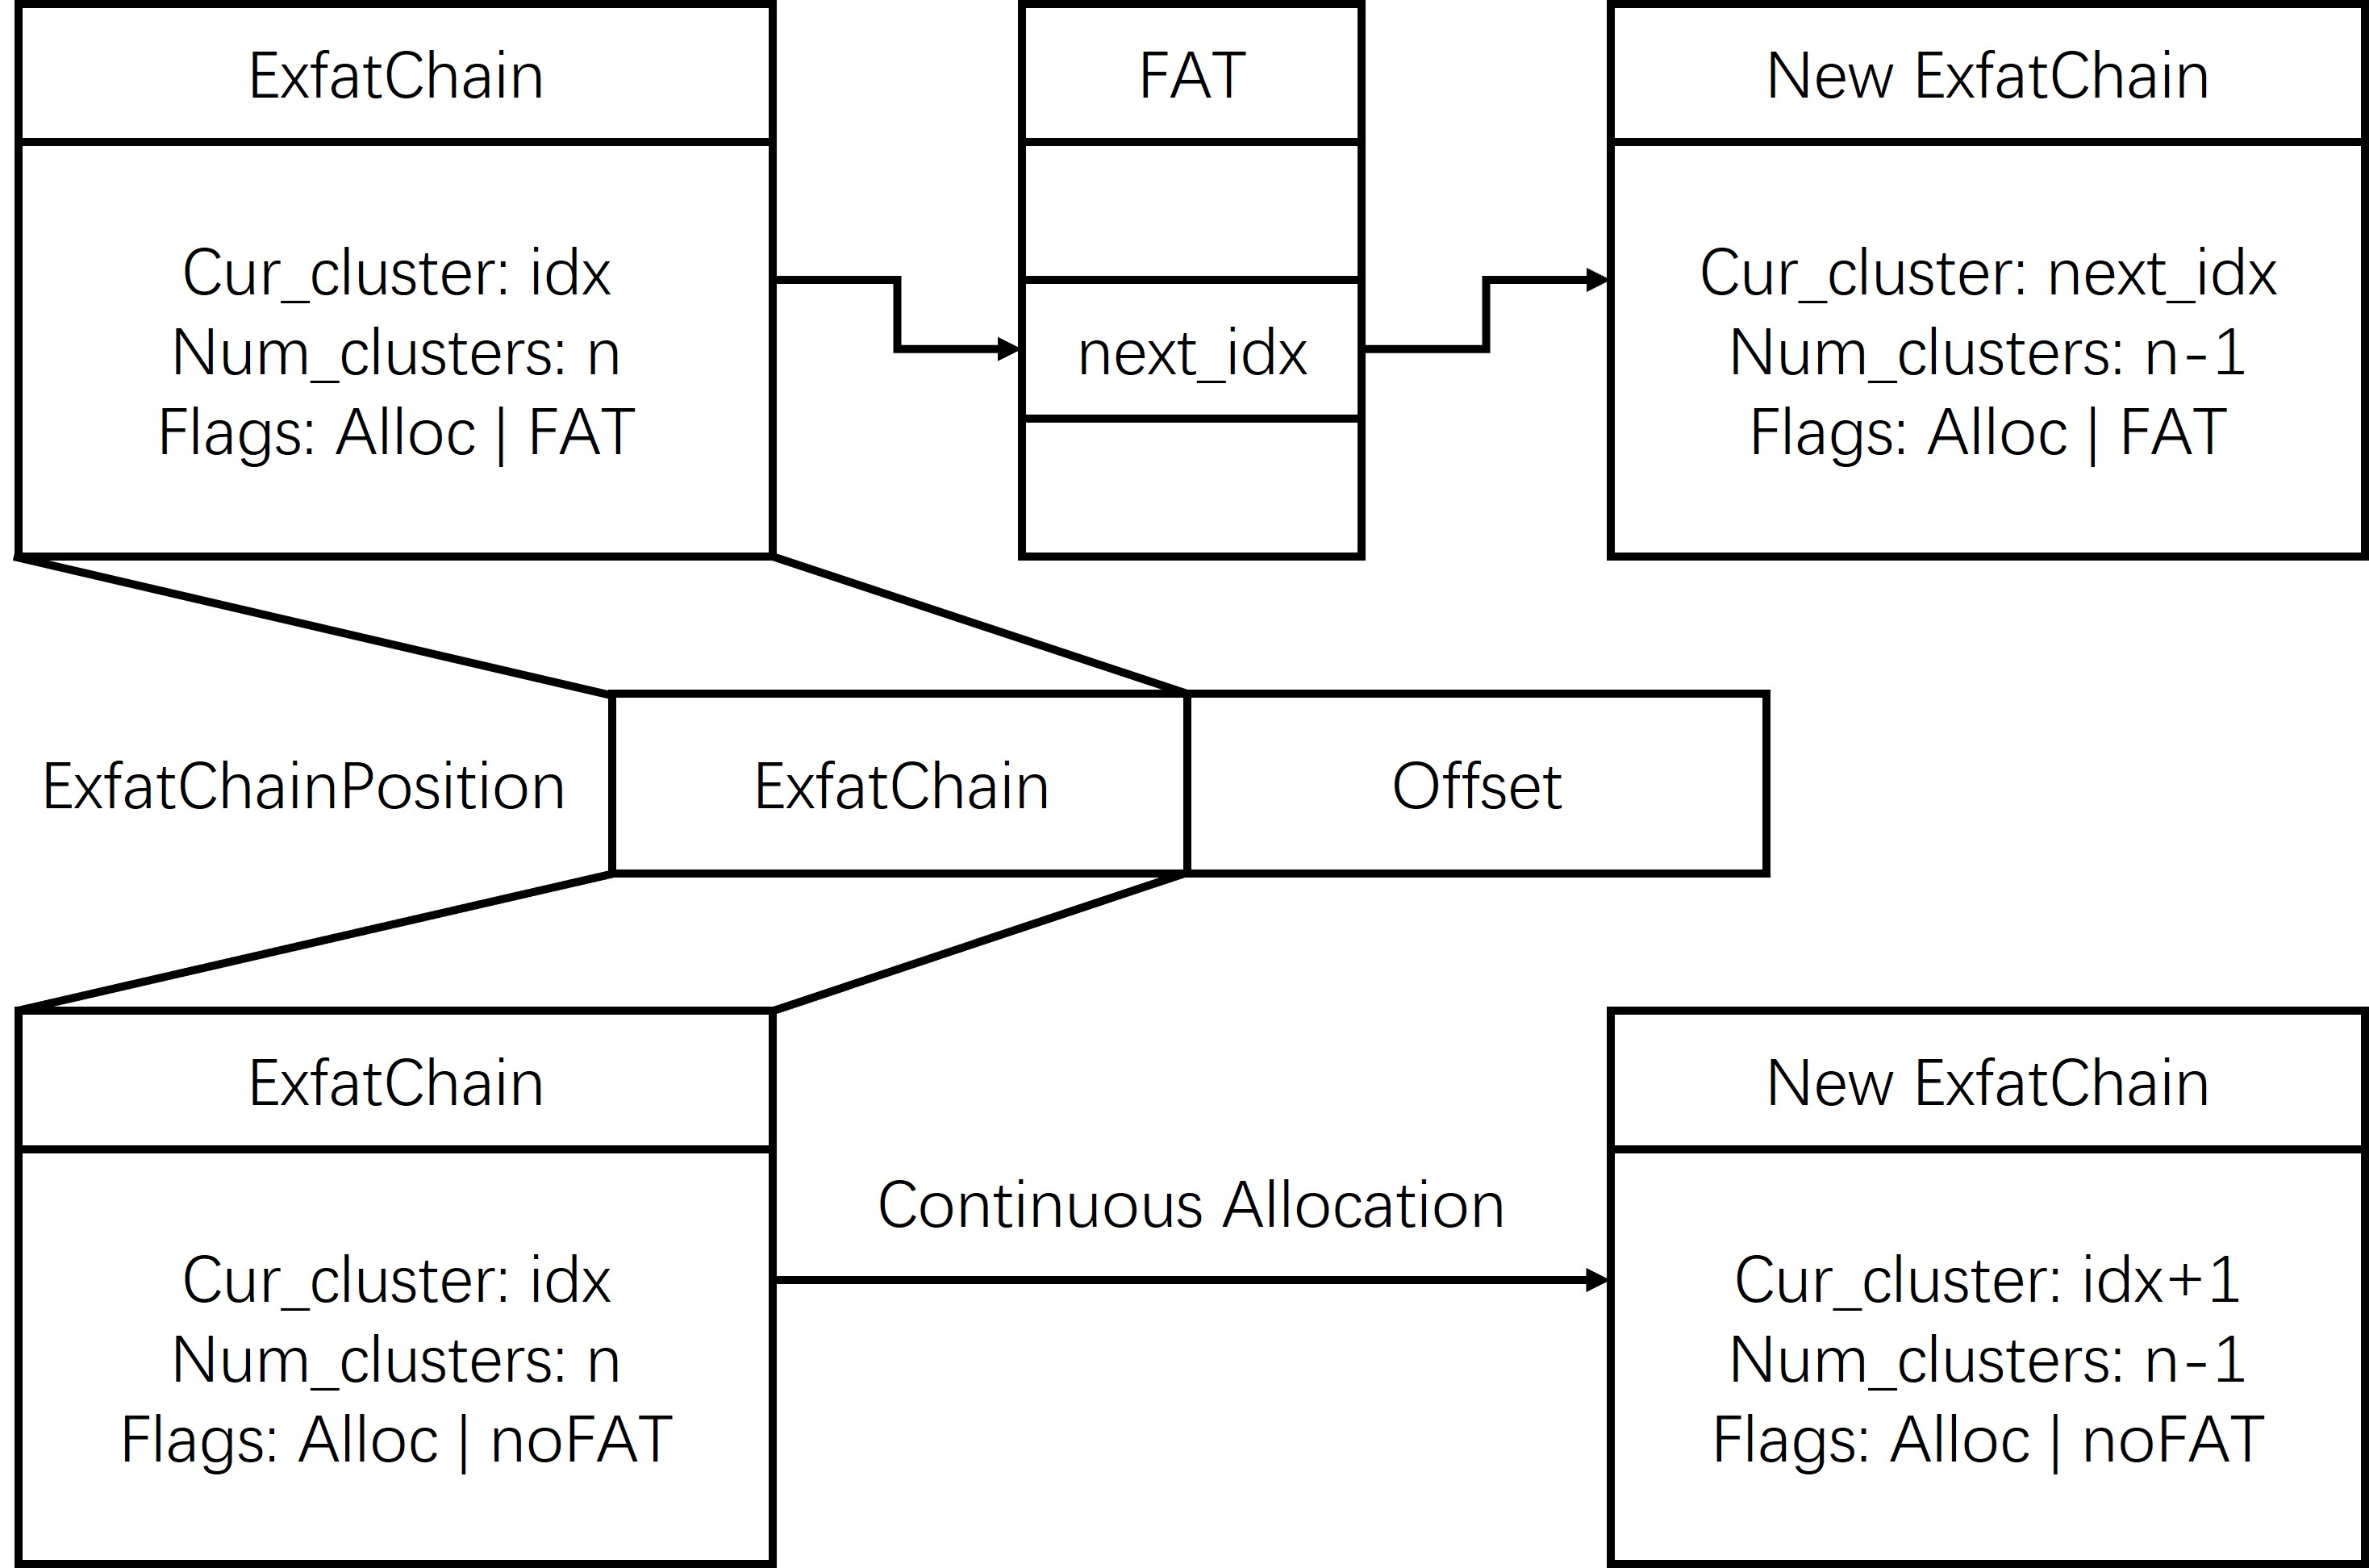
\includegraphics[width=0.8\textwidth]{chap3_cluster_chain.jpg}
    \caption{ExfatChain 寻址过程}
    \label{fig:cluster_chain}
\end{figure}

综合以上,我们把簇链抽象成 ExfatChain 结构体,使用一个二元组 (ExfatChain,Offset) 来描述数据的具体位置。
ExfatChain 结构体包含了当前簇的编号、后续合法簇的数量、文件分配方式等信息。
图\ref{fig:cluster_chain}展示了在不同分匹配模式下,使用 ExfatChain 结构进行寻址过程。
图\ref{fig:index_in_file}则展示了一个完整的数据访问过程。当应用需要访问存储设备上文件内的某个 $ offset $ 时,
通过文件的Inode内 start\_chain 字段获得文件起始簇 start\_cluster 。
访问目标的位置位于从 start\_cluster 簇开始的第 $ offset \text{ }\%\text{ } cluster\_size $ 个簇 target\_cluster 内,
簇内偏置为 $ offset \text{ }/\text{ } cluster\_size $ 。
按照图\ref{fig:cluster_chain}在描述的方式,通过文件的分配模式决定是否使用FAT表,我们可以计算出 target\_cluster 的编号。
至此,我们得到了访问目标在存储设备上的位置,访问底层设备或页缓存即可获得需要访问的数据。

\begin{figure}[h]
    \centering
    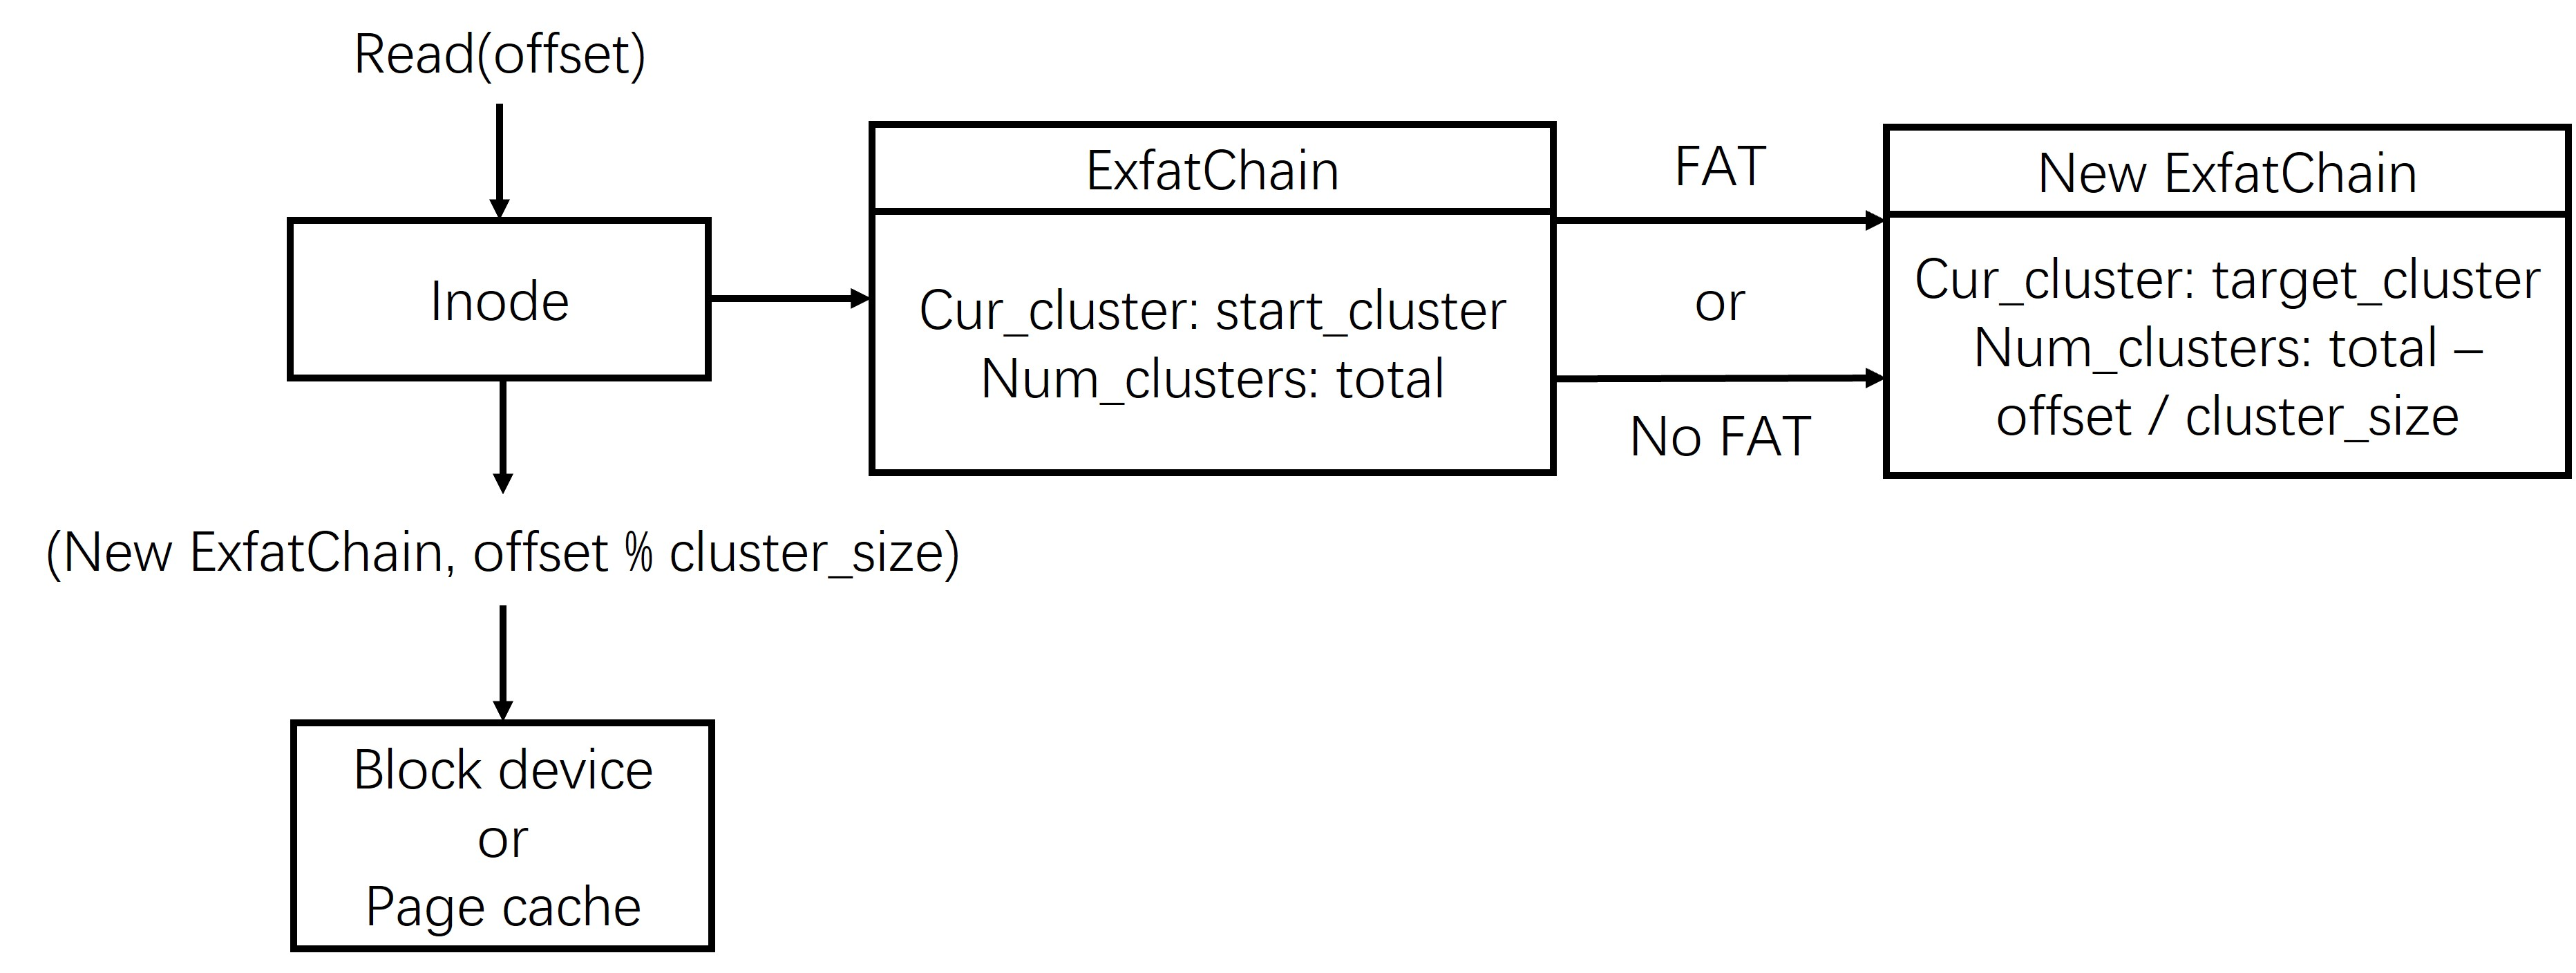
\includegraphics[width=1.0\textwidth]{chap3_index_in_file.jpg}
    \caption{文件数据访问过程}
    \label{fig:index_in_file}
\end{figure}

\section{目录的解析}\label{sec:dentry}
目录文件的文件内容是一系列目录项,一组目录项可以组成目录项集。
目录项集是对exFAT文件系统内的具体文件的抽象,exFTA内的除了根目录的每个文件都对应着一个目录项集。
这里先不讨论与大写转换表和 Bitmap 这两个特殊的系统文件对应的目录项集。
文件对应的目录项集被存储为其父目录内一组逻辑连续的目录项,分布在父目录的一段连续的逻辑地址上。
正如第二章指出的,每个目录项集由一个主目录项和一系列次目录项组成,主目录项中会指明相关联的次目录项的个数。
于是,当我们遍历一个目录的内容时,只要找到了一个主目录项,之后便可根据主目录项的信息完整的读出整个目录项集。

\begin{figure}[h]
    \centering
    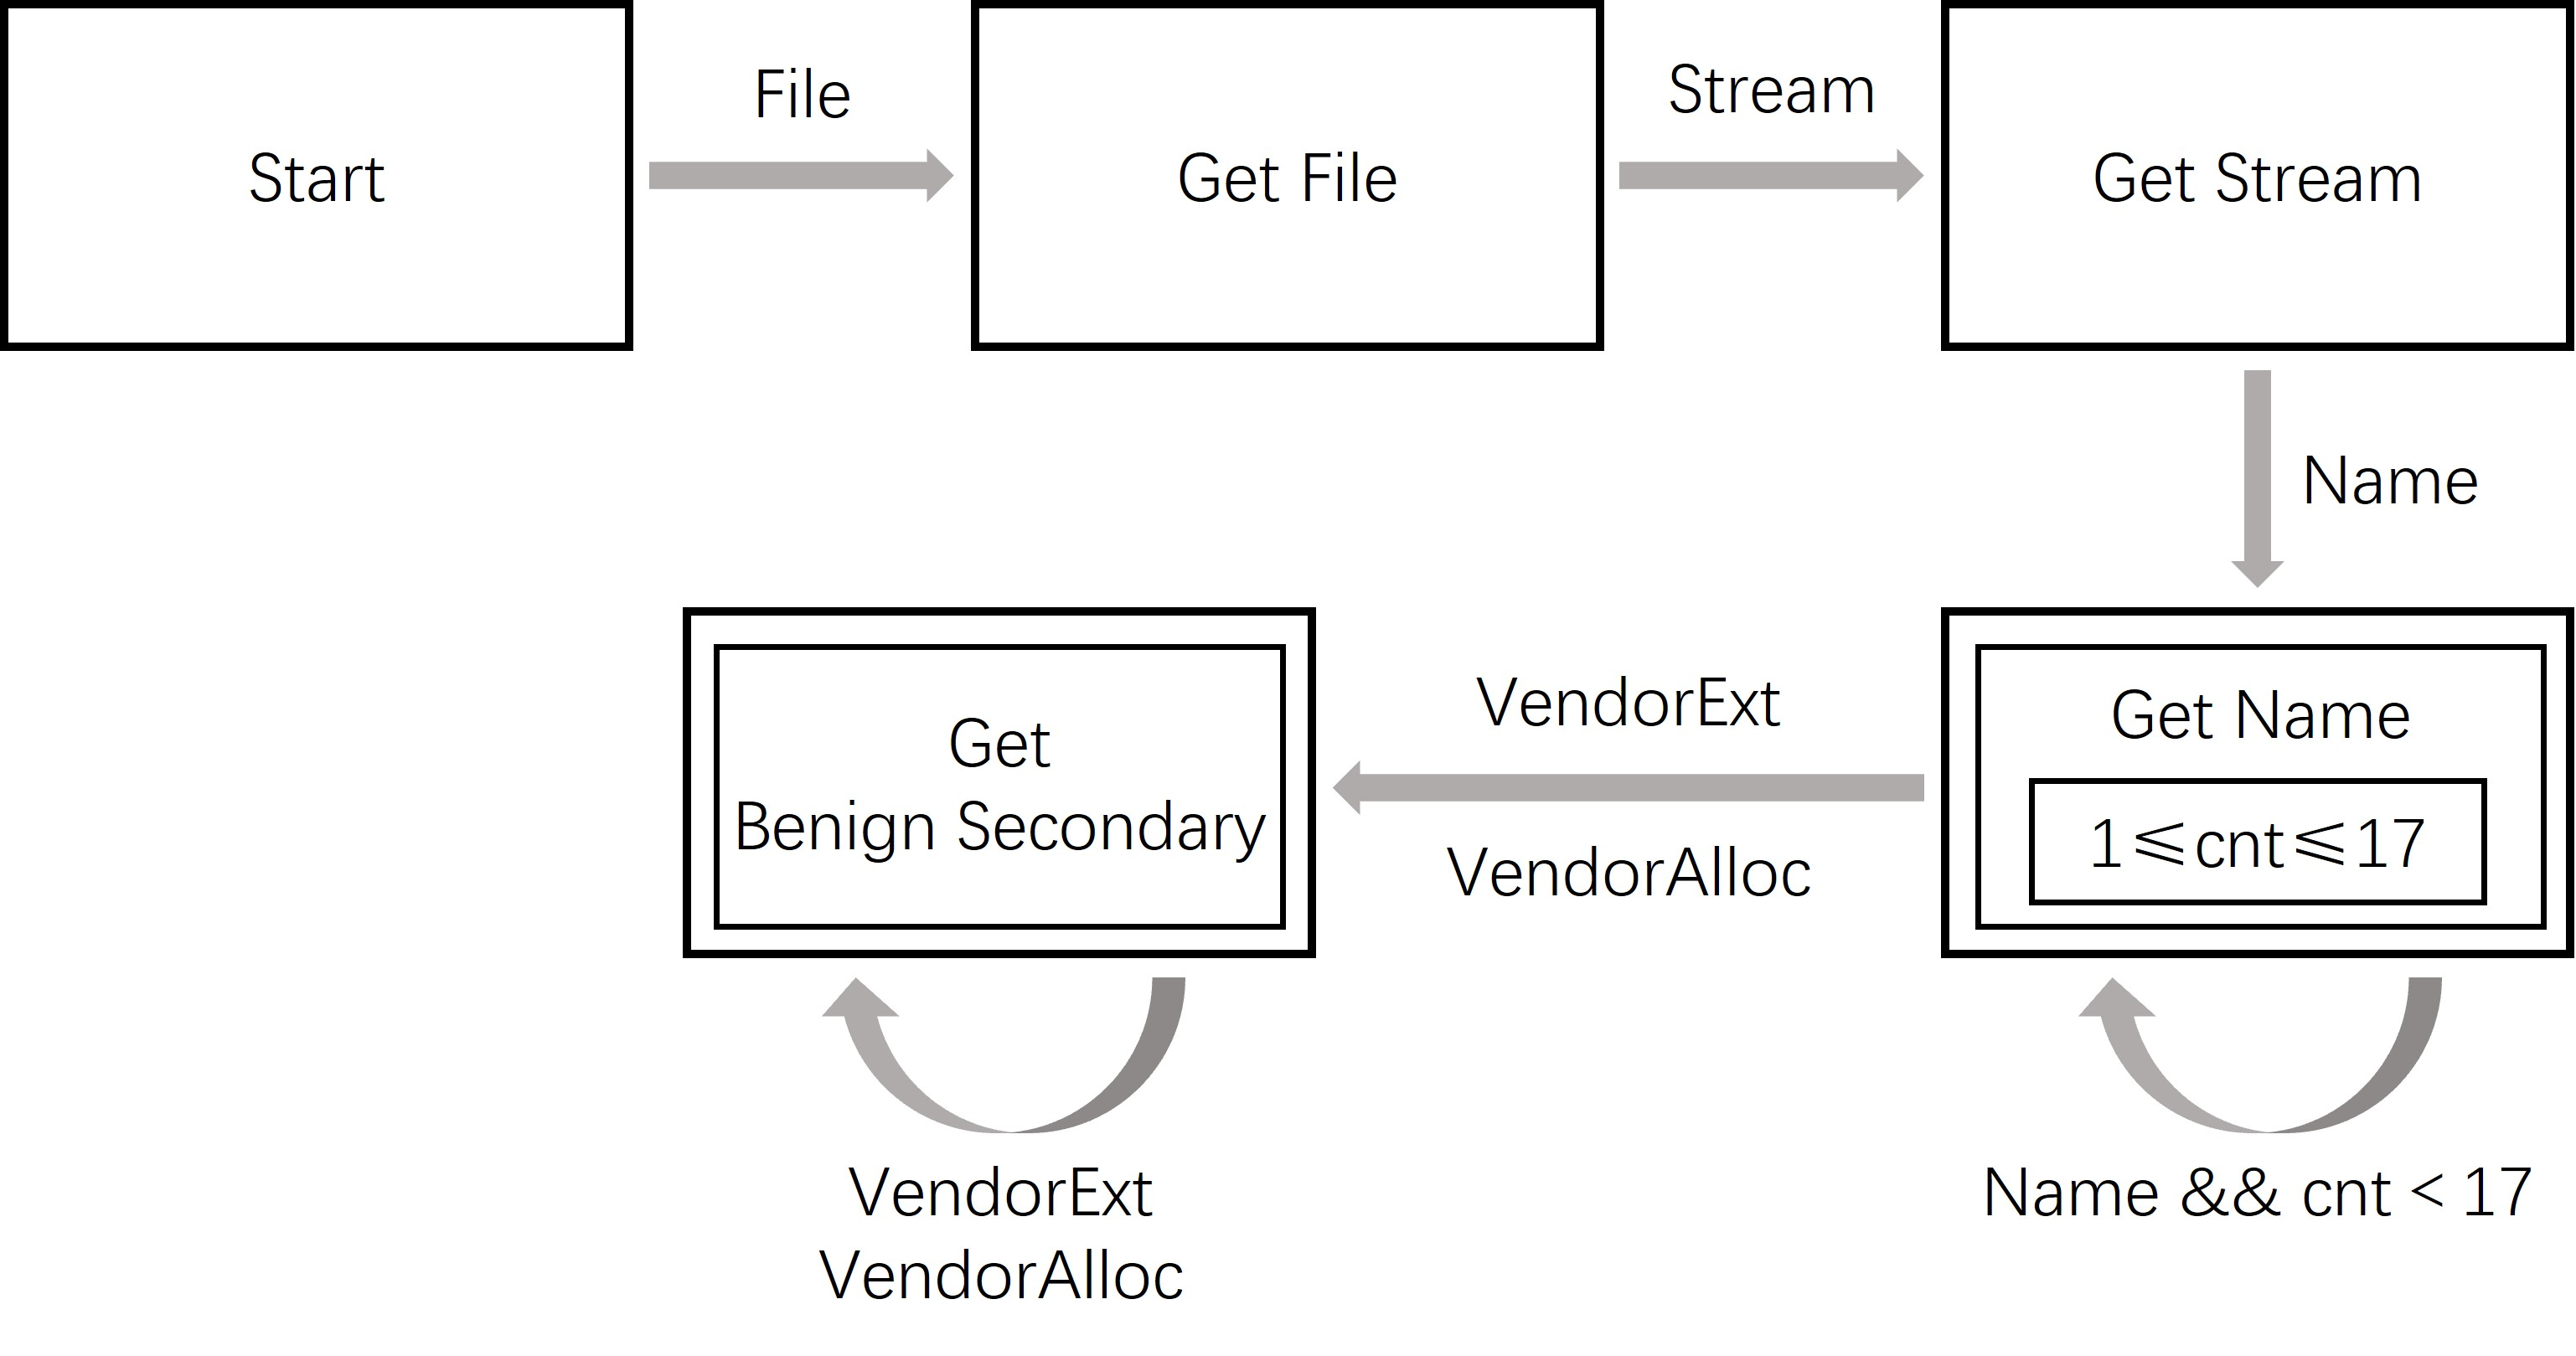
\includegraphics[width=0.8\textwidth]{chap3_dentry_state.jpg}
    \caption{目录项集解析状态机}
    \label{fig:dentry_state}
\end{figure}

读出目录项集后,需要检验其合法性。
从主目录项开始,按顺序遍历一个合法的目录项集的过程可以用一个有限状态机表示,如图\ref{fig:dentry_state}所示。
初始状态是 Start,每遇到一个新的目录项,便会根据目录项的类型转移到新状态,图中未出现的转移都是不合法的。
其中状态 GetName 包括一个参数 $ cnt $,表示当前状态下读取到的 Name 目录项的个数。
$ cnt $ 在刚进入 GetName 状态时的初始值是1,在此状态下每读到一个新的 Name 目录项,$ cnt $ 的值就增加1。
合法的终止状态包括 GetName($ 1 \leq cnt \leq max\_cnt = 17 $) 和 GetBenignSecondary。 
读出整个目录项集后,需要按顺序遍历目录项集并更新相应状态,
若遍历后到达一个合法的终止状态,则这个目录项集是合法的。


\section{大写转换表与 Bitmap}
大写转换表和 Bitmap 都是特殊的系统文件,位于根目录中,对应的目录项集均只包含一条主目录项。

大写转换表用于支持exFAT对大小写不敏感的特性,这主要是为了保证文件系统的跨平台兼容性。
exFAT的标准规定在比较两个文件名时,只要将他们都用大写转换表转换成大写后相同,就认为他们是相同的。
所以,exFAT不允许同一文件夹下存在仅通过大小写区分的文件名。
值得注意的一点是,虽然exFAT比较文件名时会使用大写转换表将文件名转化成大写,exFAT在存储文件名时
还是按照用户提供的形式存储,使用文件管理器查看时也会显示未经转换的文件名。

Bitmap 用于跟踪磁盘上的空闲簇和已分配簇,数据区中的每一个簇对应 Bitmap 中的一位,
在 Bitmap 中分别用0和1表示相应的簇未分配和已分配。
仍然需要注意的是,exFAT 中的簇的编号从2开始,而 Bitmap中的第 $ i $ 个比特代表第 $ i $ 个簇的分配状态。
故编号为 $ C $ 的簇对应 Bitmap 中的下标为 $ C - 2 $ 的比特。

\section{索引节点的实现}
索引节点,即Inode,是文件系统里最关键的组件。
作为文件在内存中的抽象,大部分和具体文件相关的系统调用都是通过 Inode 实现的。
在小节\ref{sec:FAT}和小节\ref{sec:dentry}中分别介绍了如何访问文件的内容以及如何解析目录,
在此基础上可以实现和具体文件相关的所有操作。

\begin{figure}[h]
    \centering
    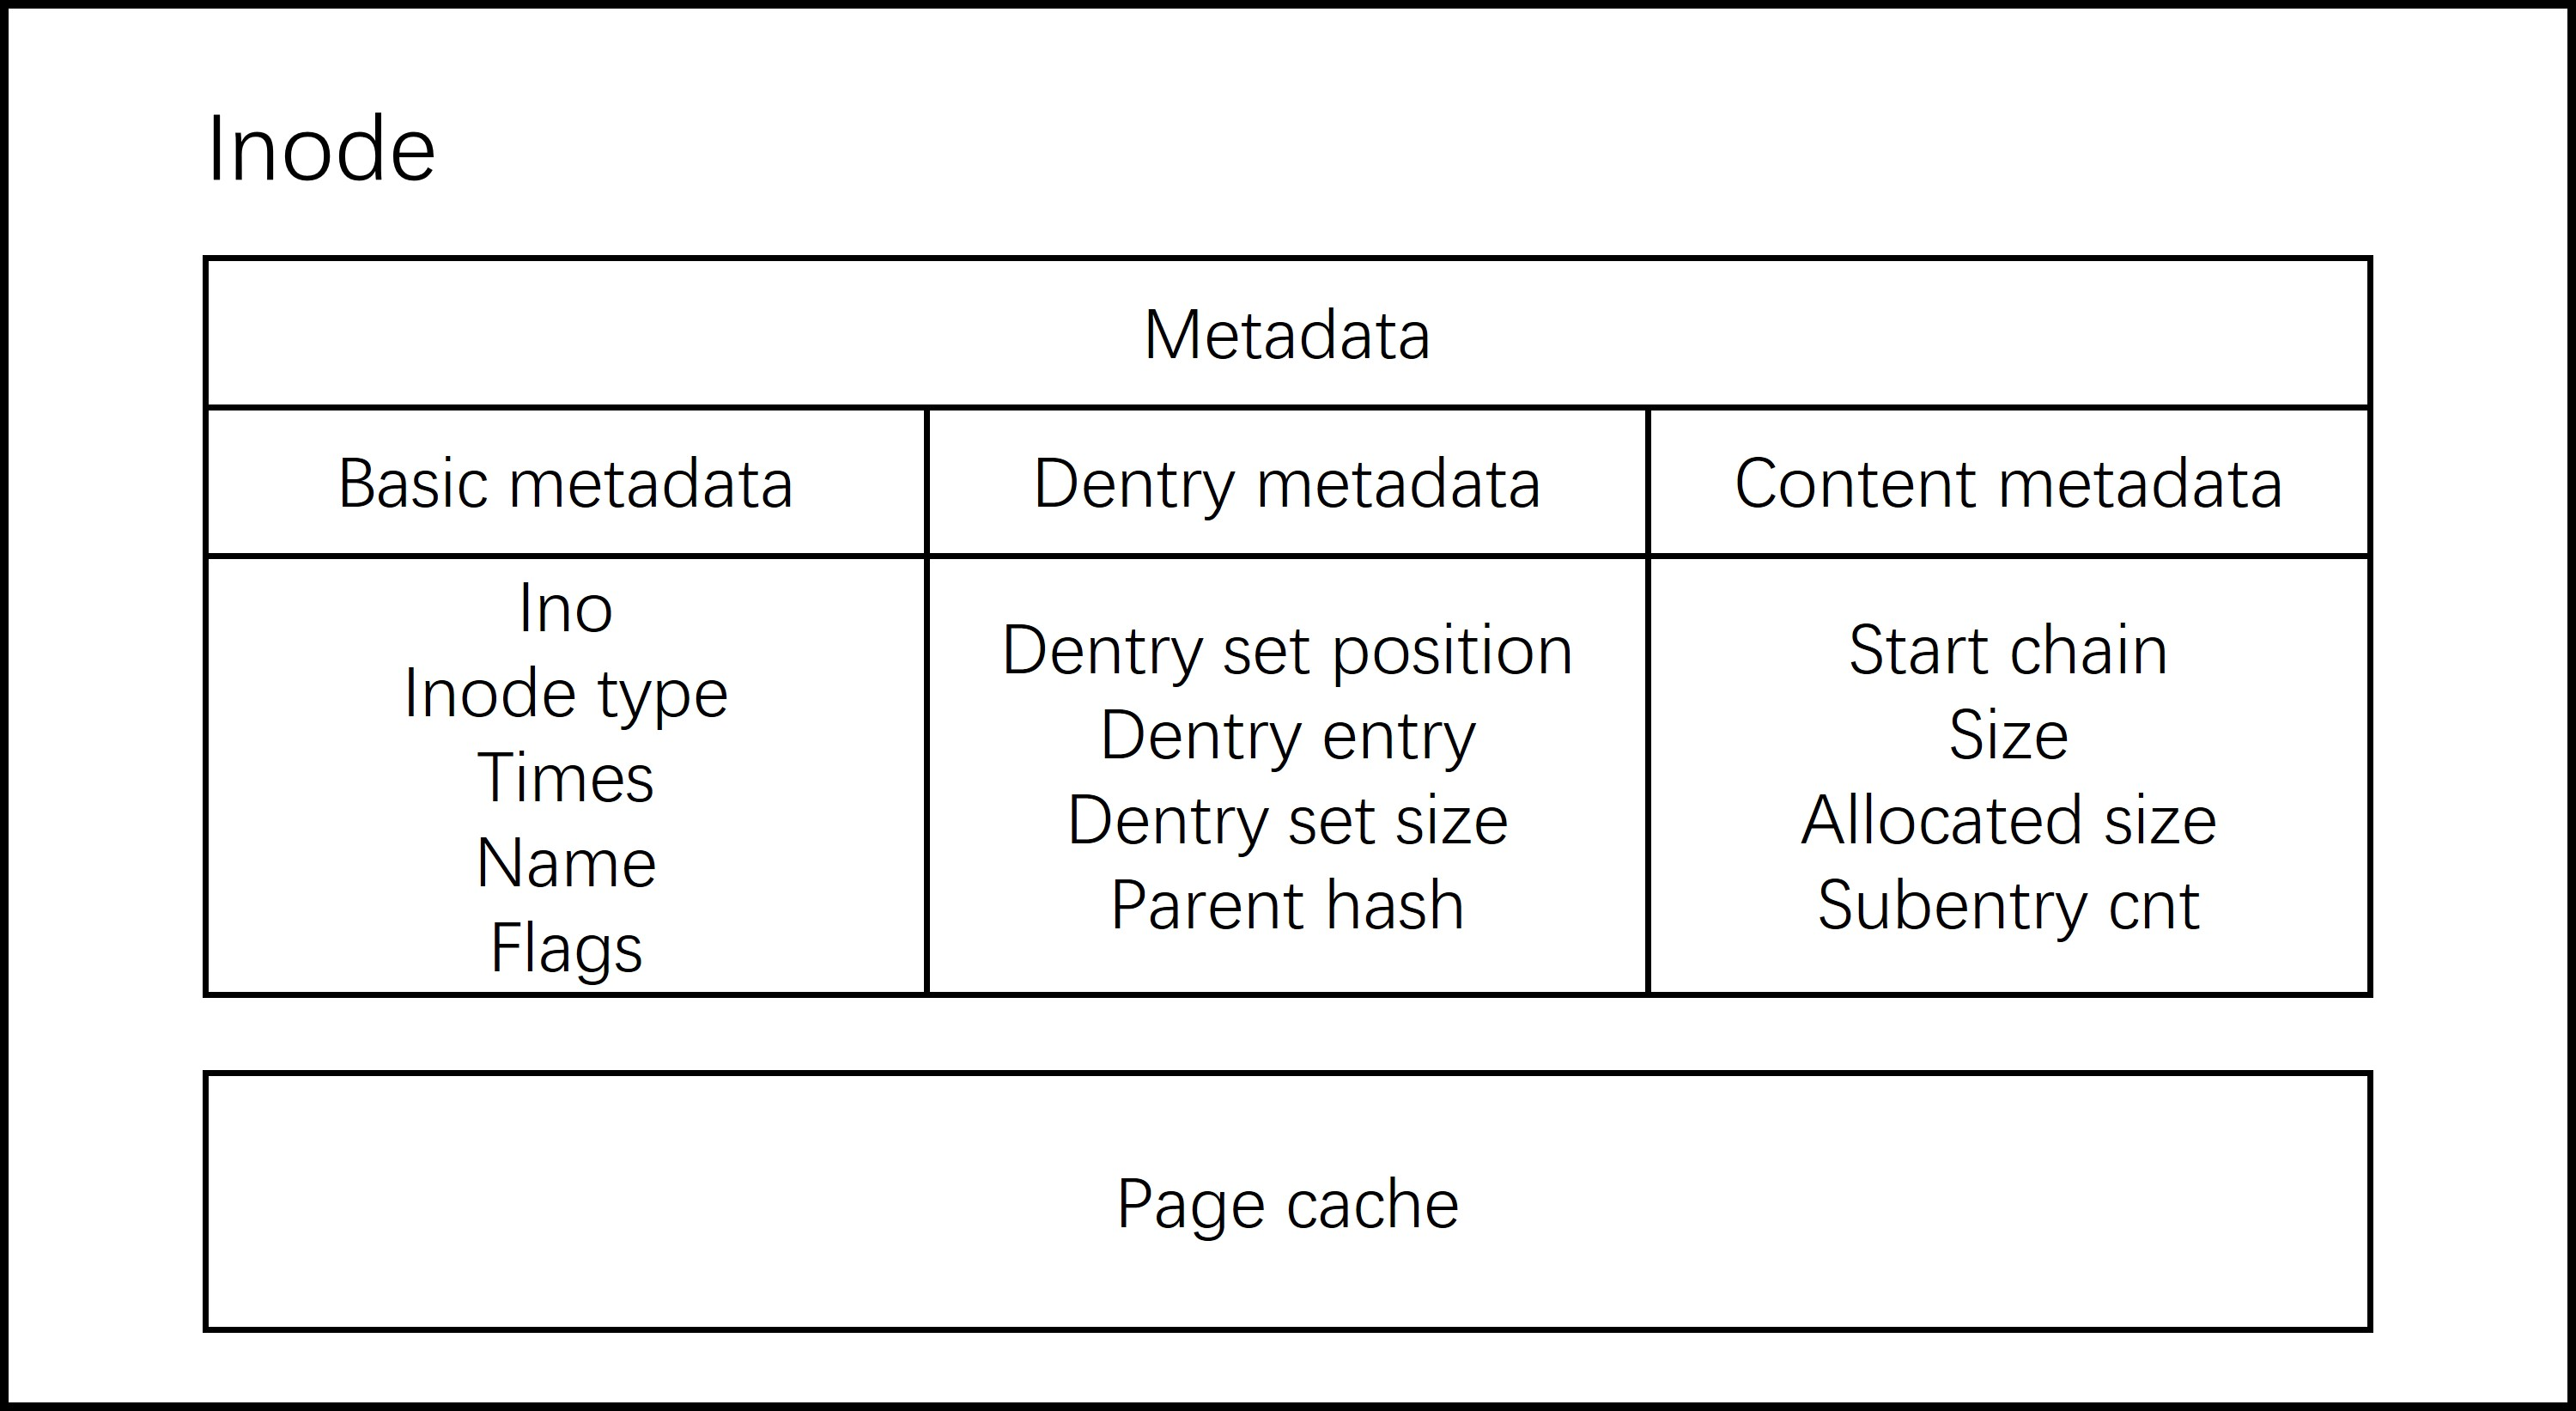
\includegraphics[width=0.8\textwidth]{chap3_inode.jpg}
    \caption{Inode 结构}
    \label{fig:inode}
\end{figure}

我们对 Inode 的设计原则是在能支持完整的文件系统功能的前提下,尽量做到精简,不存储冗余的元数据。
Inode 的结构如图\ref{fig:inode}所示,依据目的不同大致可将 Inode 的成员分为两大类:元数据、页缓存。
其中页缓存用于在内存中缓存文件内容,加速对文件内容的访问。
而元数据又可以按照根据用途不同分为三个主要部分:基本元数据(Basic metadata)、
目录项相关元数据(Dentry metadata)、文件内容元数据(Content metadata)。
下面我们将详细介绍这些元数据。
\begin{itemize}
    \item 基本元数据是和文件的基本信息相关的元数据,包括以下几个部分:
    \begin{itemize} 
        \item 索引节点编号(Ino)
        \item 文件类型(Inode type,可能出现的类型包括文件和目录)
        \item 时间戳(Times,包括创建时间、修改时间、访问时间)
        \item 文件名(Name)
        \item 文件标志位(Flags,描述文件状态,如是否为只读文件等)
    \end{itemize}
    \item 目录项元数据是和文件的目录项集相关的元数据,包括以下几个部分:
    \begin{itemize} 
        \item 目录项集在存储设备上的物理地址(Dentry set position)
        \item 目录项集在其父目录内的逻辑地址(Dentry entry)
        \item 目录项集的大小(Dentry set size)
        \item 父目录 Inode 的哈希值(Parent hash)
    \end{itemize}
    \item 文件内容元数据是和访问文件内容相关的元数据,包括以下几个部分:
    \begin{itemize} 
        \item 文件的起始簇及分配方式(Start chain)
        \item 文件内合法数据的大小(Size)
        \item 文件的分配大小(Allocated size)
        \item 子目录的数量(Subentry cnt,只对目录文件有效)
    \end{itemize}
\end{itemize}

Inode 向上层提供的接口可分为三大类:基本信息接口\ref{tab:basic}、与文件读写相关接口\ref{tab:io}、
与目录操作相关接口\ref{tab:dir}。
每个接口的功能在相应的表格中列出,功能的具体实现主要用到了本章前几节的内容,实现中特别需要注意的点也在对应的描述中标明了。

\begin{table}[h]
    \centering
    \begin{tabularx}{\textwidth}{|c|Y|}
    \hline
    接口 & 描述 \\
    \hline
    ino & 获取 Inode 编号\\
    \hline
    size & 获取文件内合法数据的大小\\
    \hline
    type\_ & 获取文件类型(普通文件、目录等)\\
    \hline
    时间类接口 & 获取或修改时间戳\\
    \hline
    权限相关接口 & 获取或修改文件权限\\
    \hline
    fs & 获取 Inode 所在文件系统引用\\
    \hline
    pagecache & 获取 Inode 内的页缓存引用\\
    \hline
    \end{tabularx}
    \caption{Inode 提供的基本信息接口}
    \label{tab:basic}
\end{table}

\begin{table}[h]
    \centering
    \begin{tabularx}{\textwidth}{|c|Y|}
    \hline
    接口 & 描述 \\
    \hline
    read\_at & 从指定位置读取数据,使用页缓存\\
    \hline
    read\_direct\_at & 从指定位置读取数据,不使用页缓存\\
    \hline
    write\_at & 向指定位置写入数据,使用页缓存\\
    \hline
    write\_direct\_at & 向指定位置写入数据,不使用页缓存\\
    \hline
    resize & 改变文件的分配大小\\
    \hline
    sync & 同步页缓存到存储设备\\
    \hline
    \end{tabularx}
    \caption{Inode 提供的与文件读写相关接口}
    \label{tab:io}
\end{table}

\begin{table}[h]
    \centering
    \begin{tabularx}{\textwidth}{|c|Y|}
    \hline
    接口 & 描述 \\
    \hline
    create & 在当前目录内创建文件或目录,不允许创建同名文件\\
    \hline
    readdir\_at & 从指定位置开始读取当前目录,列出读到的所有文件
    (默认每个目录的前两个条目别是当前目录 . 和父目录 .. )\\
    \hline
    lookup & 在当前目录内查找给定文件名,若存在,返回相应文件的 Inode\\
    \hline
    unlink & 删除当前目录内的指定文件(unlink 是针对非目录文件的接口)\\
    \hline
    rmdir & 删除当前目录内的指定目录(只允许删除空目录)\\
    \hline
    rename & 重命名文件,允许重命名到其他目录下,通过这一点也可以实现文件的移动。
    重命名是一个相对复杂的操作,可以看作是旧目录内删除相应目录项,随后在新目录内创建新的目录项\\
    \hline
    \end{tabularx}
    \caption{Inode 提供的与目录操作相关接口}
    \label{tab:dir}
\end{table}
% vim:ts=4:sw=4
